% !TeX program = xelatex
\documentclass[11pt,a4paper]{article}
\usepackage[margin=24mm]{geometry}
\usepackage{amsmath,amssymb,booktabs,array,tikz}
\usetikzlibrary{arrows.meta,positioning}
\usepackage[hidelinks]{hyperref}
\title{From Fixed Paths to an Executable Plan:\\An Assessment of Our Construction and SCALE}
\author{Internal research assessment}
\date{November 21, 2026}
\begin{document}\maketitle
\noindent\textbf{Purpose.} Compare the actual responsibilities and guarantees of
the algorithms before claiming a performance advantage or a new theoretical
result. This note audits existing code and published descriptions. It does not
implement an external solver, modify the controller, or alter the main paper.

\section{The comparison must separate three tasks}
\begin{center}
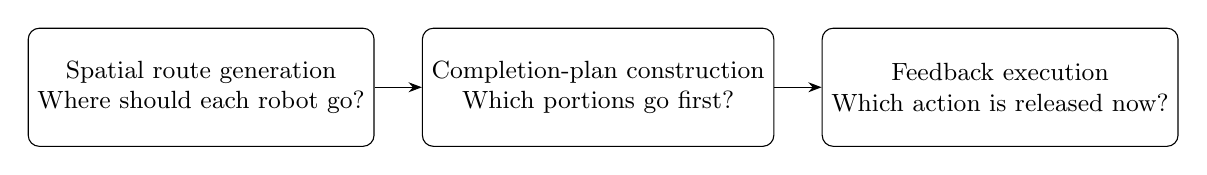
\begin{tikzpicture}[>=Stealth,box/.style={draw,rounded corners,align=center,minimum height=15mm,font=\small}]
\node[box] (route) {Spatial route generation\\Where should each robot go?};
\node[box,right=6mm of route] (order) {Completion-plan construction\\Which portions go first?};
\node[box,right=6mm of order] (exec) {Feedback execution\\Which action is released now?};
\draw[->] (route)--(order);\draw[->] (order)--(exec);
\end{tikzpicture}
\end{center}
Our fixed-path study holds spatial routes fixed. The exhaustive
\texttt{WaitDuplicationSolver} searches for a completion plan, and
\texttt{TrafficManager} executes a supplied validated plan. The optional
\texttt{plan\_builder} interface can instead supply a constructive witness.
These are distinct construction modes, not one universal search algorithm.

SCALE's route/conflict-resolution module uses graph-search MRPP methods with
SICD conflict checks. Its HAPG compiler takes feasible ranked paths as input.
Its CAPH MILP then adjusts selected passage orders over a bounded horizon [1,
Secs.~III-B, IV-A, IV-B]. Thus the complete SCALE system is not simply a MILP
alternative to our BFS. A compiler consuming a valid plan must not be compared
with a solver that is still trying to construct one.

\section{What our exhaustive solver actually guarantees}
Let a fixed route have $m_i$ edges and $m_i+1$ vertices. Its original constituent
word is
\begin{equation}
\mathcal W_i=(p_{i,0},e_{i,01},p_{i,1},\ldots,e_{i,m_i-1,m_i},p_{i,m_i}),
\qquad L_i=2m_i+1.
\end{equation}
The solver state records how many constituents have been consumed:
\begin{equation}
q=(q_1,\ldots,q_n),\quad 0\le q_i\le L_i,\qquad
|Q|\le\prod_{i=1}^n(L_i+1).
\end{equation}
For every nonempty subset of unfinished robots, a successor consumes the next
constituent for those robots; the others contribute their current point sweep.
The successor is accepted exactly when all selected movement/wait sweeps are
pairwise disjoint. No all-wait self-loop is needed for untimed reachability.

\clearpage
\subsection{Restricted completeness, not unrestricted physical completeness}
\textbf{Claim supported by the code structure.} Subject to the implemented exact
geometry predicates and valid early rejection tests, the BFS finds a witness if
one exists in this finite constituent-transition model; otherwise it exhausts
the reachable states. This is stronger than a heuristic that may simply miss
an allowed transition.

\textbf{Reason.} Every permitted transition is enumerated. The successor depends
only on the constituent counts, so one recorded predecessor per state suffices
for reachability. Each accepted edge strictly increases $\sum_i q_i$.
Consequently, the finite graph has no progress cycle, and BFS either reaches
$(L_1,\ldots,L_n)$ or finishes its queue. Its two early rejection families are
overlapping initial/final footprints and reversed endpoint order on a shared
straight line, for fixed positive-size bodies constrained to those routes.

This does \emph{not} prove completeness for every continuously timed physical
execution. The model admits waiting only at its designated vertices and requires
disjoint full sweeps within each tuple stage. It excludes exploiting precise
synchronization of overlapping sweeps, adding intermediate stopping positions,
rerouting, or changing the footprint model. An \texttt{infeasible} result is a
result about this model, not every conceivable physical maneuver.

\subsection{Cost and objective}
At most $2^n-1$ mover subsets are considered at a state. With $c_S$ bounding a
cached-sweep pair-intersection test, a simple loose search bound is
\begin{equation}
O\!\left(\prod_i(L_i+1)\;2^n n^2c_S\right),
\end{equation}
excluding geometry precomputation and assuming bounded-cost state bookkeeping.
The implementation stores predecessor rows and tuple states, adding per-state
storage proportional to $n$ beyond the number of states. This bound is not a
claim of polynomial fleet scalability.

BFS minimizes the number of tuple transitions in this particular graph. It does
\emph{not} minimize physical makespan: point consumption, translations of
different lengths, rotations, acceleration and braking do not have equal elapsed
durations. Neither transition-count optimality nor completeness establishes
novelty; product-space planning is established prior art [2,3].

\subsection{The larger demonstrations use other construction modes}
\texttt{controlled.py} calls the BFS only when no \texttt{plan\_builder} is supplied.
The incremental-routing example explicitly calls \texttt{dag\_witness}, which
constructs and validates a witness from acyclic whole-route requirements. Other
demonstrations can provide fixture-specific witnesses. Therefore, a 50-robot
execution result does not demonstrate that this exhaustive BFS solved an
unrestricted 50-robot construction problem. Construction time, validation time,
runtime control, and animation must be reported separately.

\clearpage
\section{A construction test without a supplied passage order}
We used the existing \texttt{02\_10\_RobotPath\_AlternatingProgress} routes, scaled
to metres, with the existing $1.5\times1.5$ m rectangular sweep backend. No
nominal ranks, priorities, tuple witness or passage labels were supplied.
The existing solver returned a plan and \texttt{validate} rebuilt its sweeps.
\begin{center}
\begin{tabular}{lr}\toprule
Local construction check & Result\\\midrule
Robots & 2\\
Edges per route & 5\\
Constituents per route & 11\\
Product-state upper bound & 144\\
States discovered & 128\\
Candidate transitions checked & 345\\
Witness tuple stages & 11\\
Independent witness rebuild & Passed\\\bottomrule
\end{tabular}
\end{center}
The one observed local search took approximately $0.77$ ms. Solver setup,
geometry precomputation and witness rebuilding are excluded. This single observation is
not a benchmark and supplies no comparison with any external implementation.

\textbf{A useful correction.} The returned progress sequence is
\begin{equation}
(0,0),(1,1),(2,2),\ldots,(11,11).
\end{equation}
Both robots consume their next constituent in every stage, with pairwise
disjoint stage sweeps. The previously illustrated three-block serial schedule
is valid, but alternation is not necessary for this instance. The example
demonstrates the inadequacy of requiring one robot to finish its whole route
while the other stays at its start; it does not demonstrate that only an
alternating schedule can succeed.

The stage barriers give an untimed certificate: each stage's movements may
finish at different times and then wait for the next stage. This is not an
assertion that arbitrary unsupervised timing along the full paths is safe.

\section{What SCALE solves with search, and what it solves with MILP}
\begin{enumerate}
\item \textbf{Construct/repair routes and ranked plans.} SICD supplies an
incremental conflict predicate to search-based MRPP solvers. SCALE evaluates
LaCAM*, PIBT, PBS, ECBS and CBS variants. Some of these methods have different
completeness and optimization properties; the predicate is not itself a planner.
Local planning may change the given spatial paths.
\item \textbf{Compile execution constraints.} HAPG takes feasible ranked paths
and assigns dependencies between conflicting actions. This compilation can
express our previously constructed witness, as shown in the companion note.
\item \textbf{Adjust available orders.} CAPH's MILP selects admissible capsule
orders using duration and precedence constraints. Equation (4) minimizes a sum
of horizon-terminal capsule completion times, not full-operation makespan.
Only permitted unstarted order choices may change.
\end{enumerate}

\clearpage
\section{Guarantee comparison and the research decision}
LaCAM* has completeness/eventual-optimality results for its stated finite graph
model and additive transition costs [2]. These cannot automatically be assigned
to every SCALE configuration: permitted actions, geometric predicates, local
goals, horizons and time limits affect the problem actually searched. SCALE
Remark IV.1 describes timeout-driven group splitting, horizon reduction and
retrying. The provided manuscript does not establish a general finite bound
ensuring that this complete pipeline resolves every solvable input.
This is a scope observation, not a counterexample to SCALE's execution theorem.

\begin{center}\small
\begin{tabular}{p{27mm}p{54mm}p{60mm}}\toprule
Question & Our audited component & Corresponding external component\\\midrule
Fixed paths to a completion witness & Exhaustive constituent BFS; exponential
state bound & Coordination-space search is established; SCALE's MRPP can also
change routes.\\
Known witness to dependencies & Tuple stages and preserved conflict order &
ADG/HAPG compilation from valid plans.\\
Completion under order updates & Depends on the actual controller and retained
certificate rules & SADG/CAPH give conditional feasibility/execution results.\\
Time optimization & BFS does not optimize physical makespan & CAPH MILP
optimizes a bounded-horizon completion-time sum.\\
Speed superiority & Not established & Cannot infer speed from the word MILP.\\\bottomrule
\end{tabular}
\end{center}

\paragraph{What we can honestly conclude now.}
The original comparison of ``our heuristic versus their MILP'' was misleading.
Our exhaustive test solver has a precise restricted completeness argument, but
that is a standard finite-search property. Existing dependency representations
already encode the alternating-progress witness. We have not established a new
theoretical contribution or an external performance advantage.

\paragraph{The next bounded question.}
Compare the \emph{pairwise feasibility classification and its assumptions} with
existing fixed-path coordination results: does the four-endpoint classification
give a correct, useful shortcut under a precisely stated single-interference
model? A complete BFS can serve as a finite-instance checking oracle; it cannot
replace a mathematical proof. Before expanding the manuscript or implementing
a competing system, determine whether that property is new or a direct
corollary of known coordination-space results. If it is already known, record
the equivalence and stop treating it as a novelty claim.

\begin{thebibliography}{9}\small
\bibitem{scale} B. Cao, ``From Real-Time Planning to Reliable Execution:
Scalable Coordination for Heterogeneous Multi-Robot Fleets in Industrial
Environments,'' arXiv:2607.00591v2, 2026.
\url{https://arxiv.org/html/2607.00591v2}.
\bibitem{lacam} K. Okumura, ``Improving LaCAM for Scalable Eventually Optimal
Multi-Agent Pathfinding,'' IJCAI, 243--251, 2023.
\url{https://www.ijcai.org/proceedings/2023/0028.pdf}.
\bibitem{segment} A. Coskun, J. M. O'Kane, and M. Valtorta, ``Deadlock-Free
Online Plan Repair in Multi-robot Coordination with Disturbances,'' FLAIRS,
2021. Related Work and coordination-space formulation.
\url{https://jokane.net/pubs/CosOKaVal21.pdf}.
\end{thebibliography}
\end{document}
